\documentclass[11pt]{article}
\usepackage{amsmath,textcomp,amssymb,geometry,graphicx,float,mathrsfs,tabularx}

\def\Login{ee121-af} % Your login
\def\HW{2} % Homework number

\title{EE 121 -- Fall 2013\\Homework 2}

\markboth{EE 121 -- Fall 2013 Homework \HW}{EE 121 -- Fall 2013 Homework \HW}
\pagestyle{myheadings}

\begin{document}
\maketitle
\noindent\textbf{Team Bitdiddlers} \\
\text{Jeff Lievense, Rishi Sharma, Nader Behdin, Tim Brown}

\begin{enumerate}
  % Have a new \item for each problem
  % Make sure you have a \newpage after each item


  % PROBLEM 1
  \item
    \begin{enumerate}


        %part a)
        \item
            The probability of error on a symbol is equal to the probability of getting at least one bit-error in the $j$ bits that make up the symbol. The complement of "at least one bit-error" is "no bit errors", and the probability of that event is simply $(1 - p)^j$. Then the probability of error on a symbol is the complement of that, and we see:
            \begin{flalign*}
                P_{\mathcal{E},\mbox{sym}} &= 1 - (1 - p)^j
            \end{flalign*}


        % part b)
        \item
            To determine the probability of error, we first need to define what an error is in this new coding scheme. We say an error occurs if we are unable to properly decode a received message, and since we are using a Reed-Solomon code, we know this occurs when more than $E$ symbol errors occur -- $E$ is the maximum number of errors allowed by the Reed-Solomon code. If $k$ is the number of symbols in our raw message and $n = 2^j$ is the number of symbols in the encoded message, we can find $E$ via the following relationship:
            \begin{flalign*}
                n &= k + 2E \\
                E &= \frac{n - k}{2}
            \end{flalign*}
            We now define $N$ to be a random variable representing the total number of symbol errors in a received code message. We then define another random variable $X_i$:
            \begin{displaymath}
            X_{i} = \left\{
            \begin{array}{lr}
            1, \mbox{ if the $i^{\mbox{th}}$ symbol in the received message is corrupt} \\
            0, \mbox{ otherwise}
            \end{array}
            \right.
            \end{displaymath}

            It follows that:
            \begin{flalign*}
            N &= \sum_{i = 1}^n X_i
            \end{flalign*}

            Since the $X_i$s are Bernoulli random variables, $N$ is distributed Binomially ($N \sim \mbox{ Binom}(n,1 - (1 - p)^j)$), and we can now find the probability of error:
            \begin{flalign*}
                P_{\mathcal{E},\mbox{total}} &= P(N > E) \\
                &= \sum_{i = E + 1}^n {n\choose i}\cdot (P_{\mathcal{E},\mbox{sym}})^i \cdot (1 - P_{\mathcal{E},\mbox{sym}})^{n - i} \\
                &= \sum_{i = E + 1}^n {n\choose i}\cdot (1 - (1 - p)^j)^i \cdot ((1 - p)^j)^{n - i}
            \end{flalign*}


        % part c)
        \item
            The CLT says that, as $n$ grows large, $N$ looks Gaussian. So, if we normalize $N$ to a zero mean, unit variance Gaussian, we can approximate the probability of error $P(N > E)$ with the Q-function (the tail probability of the standard normal distribution). We define a new random variable $Z$ as follows:
            \begin{flalign*}
                Z &= \frac{N - \mathbb{E}[N]}{\sqrt{\mbox{Var}[N]}} \\
                \mathbb{E}[N] &= n\cdot P_{\mathcal{E},\mbox{sym}} \\
                \mbox{Var}[N] &= n\cdot P_{\mathcal{E},\mbox{sym}}\cdot(1 - P_{\mathcal{E},\mbox{sym}})
            \end{flalign*}
            We see that $Z$ is distributed as a standard normal, so:
            \begin{flalign*}
            P_{\mathcal{E},\mbox{total}} &= P(N > E) \\
            &= P(Z\cdot\sqrt{\mbox{Var}[N]} + \mathbb{E}[N] > E) \\
            &= P(Z > \frac{E - \mathbb{E}[N]}{\sqrt{\mbox{Var}[N]}}) \\
            &\approx Q\left(\frac{E - \mathbb{E}[N]}{\sqrt{\mbox{Var}[N]}}\right) \\
            &\approx Q\left(\frac{\frac{n - k}{2} - n\cdot(1 - (1 - p)^j)}{\sqrt{n\cdot (1 - (1 - p)^j)\cdot(1 - p)^j}}\right)
            \end{flalign*}





        % part d)
        \item
            The probability of error approaches 1 as $j$ gets large! This makes sense, since a symbol is corrupt if a single bit is flipped -- more bits means it's more likely for at least one of them to get flipped (see Figure 1).

             \begin{figure}[H]
                \begin{center}
                    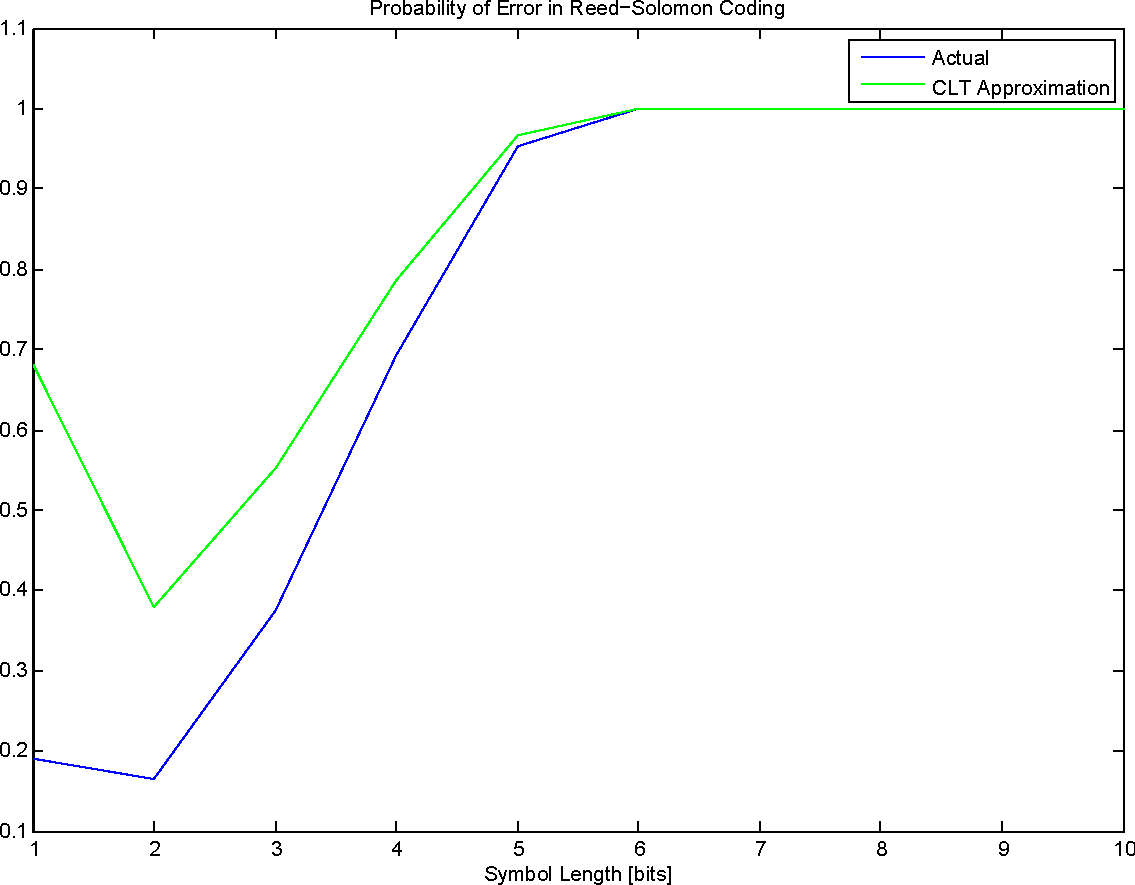
\includegraphics[width = 0.8\textwidth]{q1d.pdf}
                    \caption{}
                \end{center}
            \end{figure}



        % part e)
        \item
            In Figure 2, we see that as the probability of a single bit-error increases, the number of bits we can use to represent a symbol drops to one -- this fits with what we found in the previous question. \\
            \\
            In Figure 3, we plot the overall probability of error that results from using the optimal number of bits per symbol. As expected, it goes to one as the probability of a single bit-error increases.



            \begin{figure}[H]
                \begin{center}
                    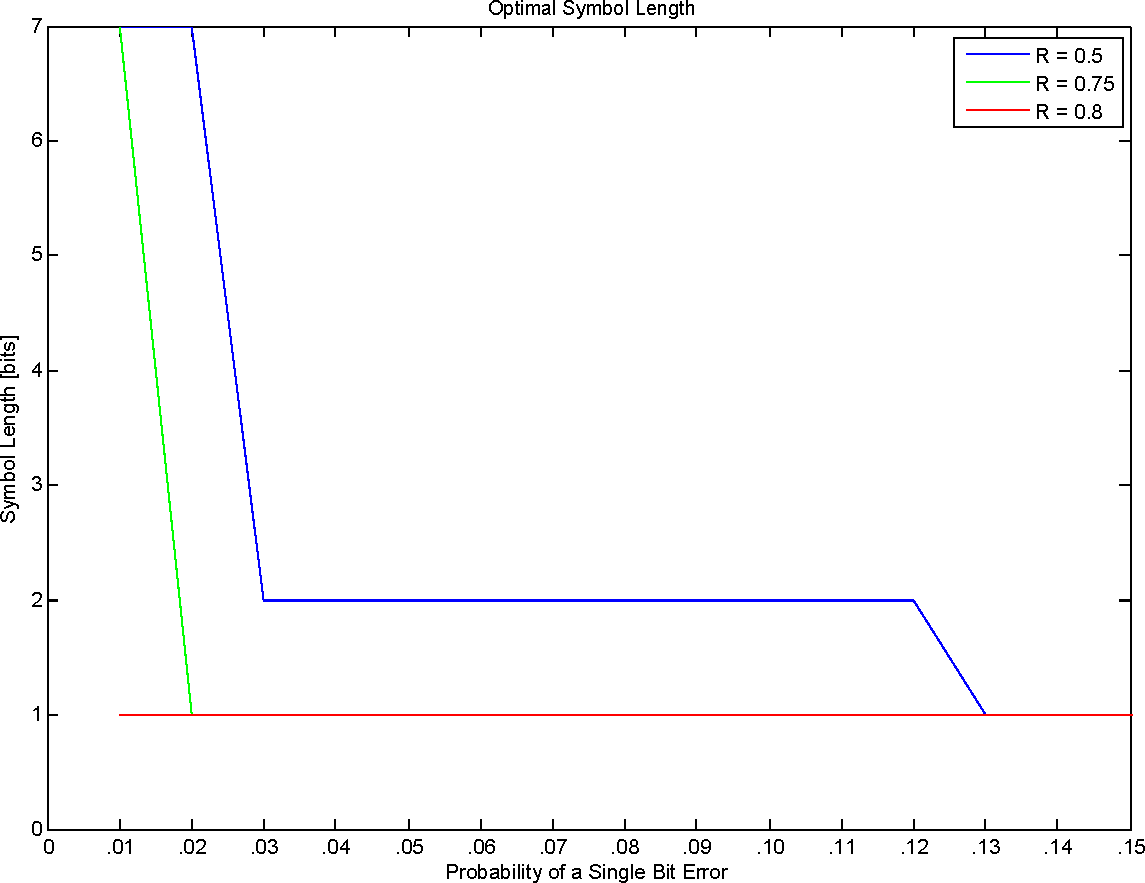
\includegraphics[width = 0.65\textwidth]{comparing_symbol_lengths.pdf}
                    \caption{}
                \end{center}
            \end{figure}

            \begin{figure}[H]
                \begin{center}
                    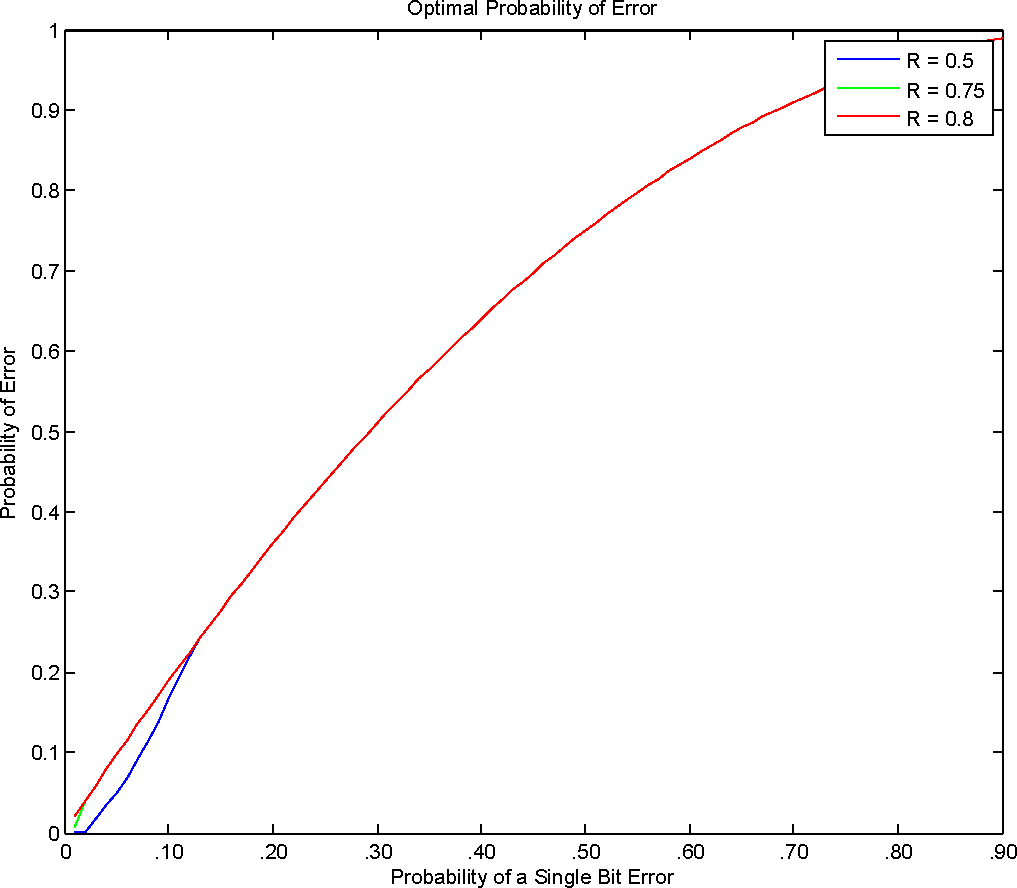
\includegraphics[width = 0.65\textwidth]{comparing_rates.pdf}
                    \caption{}
                \end{center}
            \end{figure}


            % part f)
            \item
                The Reed-Solomon code works reasonably well for low rates and very low probabilities of single bit-errors, but the probability of error blows up as the rate and bit-error probability increase.



            % part g)
            \item
                Given black-box access to a code that maps $j$ bits to $\frac{3}{2}j$ bits and decodes them, here is how our new "concatenated code" would work:
                \begin{itemize}
                    \item
                        Use a Reed-Solomon code to map $kj$ message bits ($k$ symbols) to $\frac{4}{3}kj$ "intermediate code" bits ($\frac{4}{3}k$ symbols)
                    \item
                        Take each $j$-bit symbol of the $\frac{4}{3}k$ symbols in this intermediate code and encode as a $\frac{3}{2}j$-bit symbol via the "small" code, resulting in $\frac{4}{3}k\cdot\frac{3}{2}j = 2kj$ code bits.
                    \item
                        Decoding is then performed by breaking up a $2kj$-bit received message into $\frac{3}{2}j$-bit symbols, decoding each one into a $j$-bit symbol via the "small" code, then decoding the resulting $\frac{4}{3}kj$-bit Reed-Solomon code into a $kj$-bit message via the Berlekamp-Welch algorithm.
                \end{itemize}
                We see that, in this concatenated code, $kj$ message bits are mapped to $2kj$ codebits, resulting in a rate of $R = \frac{kj}{2kj} = \frac{1}{2}$. Note that this new code can tolerate a different number of errors than the straightforward Reed-Solomon code -- if $E$ is the maximum number of tolerable errors, we have:
                \begin{flalign*}
                    \frac{4}{3}k &= k + 2E \\
                    E &= \frac{1}{6}k
                \end{flalign*}



                % part h)
                \item
                We can use the same expression for the overall probability of error in the concatenated code case as the one used in the straightforward Reed-Solomon case if we take into account which parameters change when we use the concatenated code:
                \begin{itemize}
                    \item The encoded message now contains $\frac{4}{3}k$ symbols, so $n = \frac{4}{3}k$.
                    \item $E = \frac{1}{6}k$, as shown above.
                    \item The "small" code gives us $P_{\mathcal{E},\mbox{sym}} = e^{-K_pj}$.
                \end{itemize}
                So we have:
                \begin{flalign*}
                P_{\mathcal{E},\mbox{total}} &= P(N > E) \\
                &= \sum_{i = E + 1}^n {n\choose i}\cdot (P_{\mathcal{E},\mbox{sym}})^i \cdot (1 - P_{\mathcal{E},\mbox{sym}})^{n - i} \\
                &= \sum_{i = \frac{1}{6}k + 1}^{\frac{4}{3}k} {\frac{4}{3}k\choose i}\cdot(e^{-K_pj})^i \cdot(1 - e^{-K_pj})^{\frac{4}{3}k - i}
                \end{flalign*}

    \end{enumerate}
    \newpage




  % PROBLEM 2
  \item
    \begin{enumerate}

        % part a)
        \item
            Let
            \begin{displaymath}
                N_i = \left\{
                \begin{array}{lr}
                    1 , & \mbox{if $X_i = a$} \\
                    0, & \mbox{if $X_i = b$}
                \end{array}
                \right.
            \end{displaymath}

            \begin{flalign*}
                P(N_i = 1) &= \frac{2}{3} \\
                P(N_i = 0) &= \frac{1}{3}
            \end{flalign*}
            Note that $N_i$ is a Bernoulli random variable with parameter $p = P(N_i = 1) = \frac{2}{3}$. If $N_a$ is the total number of "$a$"s in the string $\mathbf{X}^n$, then we can define $N_a$ as follows:
            \begin{flalign*}
                N_a = \sum_{i = 1}^n N_i
            \end{flalign*}
            Since $N_a$ can be written as a sum of $n$ Bernoulli random variables with parameter $p$, $N_a$ is a Binomial random variable: $N_a \sim \mbox{ Binom}(n,p)$.

        % part b)
        \item
            Since $W(X_i) = -\log_2\left(\frac{2}{3}\right)$ if $X_i = a$ and $W(X_i) = - \log_2\left(\frac{1}{3}\right)$ if $X_i = b$, we can write:
            \begin{flalign*}
            W(\mathbf{X}^n) &= \sum_{i = 1}^n W(X_i) \\
            &= -\log_2\left(\frac{2}{3}\right)\cdot(\mbox{number of "$a$"s in $\mathbf{X}^n$}) - \log_2\left(\frac{1}{3}\right)\cdot(\mbox{number of "$b$"s in $\mathbf{X}^n$}) \\
            &= -\log_2\left(\frac{2}{3}\right)\cdot N_a - \log_2\left(\frac{1}{3}\right)\cdot(n - N_a) \\
            &= -N_a - n\cdot\log_2(\frac{1}{3})
            \end{flalign*}


        % part c)
        \item
            On average, we expect there to be $\mathbb{E}[N_a] = n\cdot\mathbb{E}[N_i]$ "$a$"s in a "typical" string, so we define the typical set to be the set of strings containing between $n(\mathbb{E}[N_i] - \epsilon) = n(\frac{2}{3} - \epsilon)$ and $n(\mathbb{E}[N_i] + \epsilon) = n(\frac{2}{3} + \epsilon)$ "$a$"s, that is:
            \begin{flalign*}
                T_{\epsilon}^n &= \{\mathbf{x}^n : n\beta \leq N_a(\mathbf{x}^n) \leq n\alpha\} \\
                               &= \{\mathbf{x}^n : n(\frac{2}{3} - \epsilon) \leq N_a(\mathbf{x}^n) \leq n(\frac{2}{3} + \epsilon)\} \\
            \end{flalign*}
            And thus we have, for $\epsilon = \frac{1}{10}$:
            \begin{flalign*}
                \beta &= \frac{2}{3} - \frac{1}{10} = \frac{17}{30} \approx 0.567 \\
                \alpha &= \frac{2}{3} + \frac{1}{10} = \frac{23}{30} \approx 0.767
            \end{flalign*}

        % part d)
        \item
            We can calculate $P(\{T_{\epsilon}^n\})$ exactly by calculating the probability of $N_a$ being between $\lceil n\beta \rceil$ and $\lfloor \alpha \rfloor$. Since $N_a$ is a Binomial random variable, we have:
            \begin{flalign*}
                P(\{T_{\epsilon}^n\}) &= P(\lceil n\beta \rceil \leq N_a \leq \lfloor n\alpha \rfloor) \\
                &= \sum_{i = \lceil n\beta \rceil}^{\lfloor n\alpha \rfloor} {n\choose i}\cdot P(X_i = a)^i \cdot P(X_i = b)^{n - i} \\
                &\approx 0.9667
            \end{flalign*}
            Similar to part (c) of question one, we can approximate $P(\{T_{\epsilon}^n\})$ by using the CLT to say that $N_a$ is approximately Gaussian. Recall that $Z = \frac{N_a - \mathbb{E}[N_a]}{\sqrt{\mbox{Var}[N_a]}}$ is a random variable representing the "standard normalization" of $N_a$, and $\Phi(x)$ is the cumulative distribution function of the standard normal:
            \begin{flalign*}
                P(\{T_{\epsilon}^n\}) &= P(\lceil n\beta \rceil \leq N_a \leq \lfloor n\alpha \rfloor) \\
                &= P\left(\frac{\lceil n\beta \rceil - n\mathbb{E}[N_a]}{\sqrt{\mbox{Var}[N_a]}} \leq Z \leq \frac{\lfloor n\alpha \rfloor - n\mathbb{E}[N_a]}{\sqrt{\mbox{Var}[N_a]}}\right) \\
                &\approx \Phi(\frac{\lfloor n\alpha \rfloor - n\mathbb{E}[N_a]}{\sqrt{\mbox{Var}[N_a]}}) - \Phi(\frac{\lceil n\beta \rceil - n\mathbb{E}[N_a]}{\sqrt{\mbox{Var}[N_a]}}) \\
                &\approx 0.9560
            \end{flalign*}


        % part e)
        \item
            If we have a bag of marbles that weighs at most one pound and we know each marble weighs at least $\frac{1}{x}$ pounds, then there are at most $\frac{1}{\frac{1}{x}} = x$ marbles in the bag. \\
            \\
            We will now draw a parallel between this marble analogy and the typical set. We will view marbles as strings, and their weights as probabilities. The WLLN tells us that as $n \rightarrow \infty$, $P(\{T_{\epsilon}^n\}) \rightarrow 1$, so the typical set "weighs" at most one. We can get the "weight" of the lightest string from the definition of the typical set:
            \begin{flalign*}
                T_{\epsilon}^n &= \{\mathbf{x}^n : 2^{-n(H(X) + \epsilon)} \leq p_X(\mathbf{x}^n) \leq 2^{-n(H(X) - \epsilon)} \}
            \end{flalign*}
                We see that the "weight" (probability) of any string in the typical set ($p_X(\mathbf{x}^n)$) has a lower bound of $2^{-n(H(X) + \epsilon)}$. Thus, regardless of $n$ and $\epsilon$, the typical set can contain at most $\frac{1}{2^{-n(H(X) + \epsilon)}}$ strings. That is:
                \begin{flalign*}
                    |T_{\epsilon}^n| &\leq 2^{n(H(X) + \epsilon)}
                \end{flalign*}

        %part f)
        \item
            We can calculate $|T_{\epsilon}^n|$ exactly by simply counting the number of strings in the typical set:
            \begin{flalign*}
               |T_{\epsilon}^n| &= \sum_{i = \lceil n\beta \rceil}^{\lfloor n\alpha \rfloor} {n\choose i} \\
               &\approx 1.2255\cdot10^{29}
            \end{flalign*}
            The upper bound approximation we found via the marble analogy yields:
            \begin{flalign*}
            |T_{\epsilon}^n| &\leq 2^{n(H(X) + \epsilon)} \\
            &\approx 4.5057\cdot10^{30}
            \end{flalign*}


        %part g)
        \item



    \end{enumerate}
    \newpage


  % PROBLEM 3
  \item

    \newpage


  % PROBLEM 4
  \item

    \newpage


  % PROBLEM 5
  \item

    \newpage
\end{enumerate}
\end{document} 